\documentclass{article}
\usepackage{graphicx} % Required for inserting images
\usepackage{multicol}
\usepackage{geometry}
\usepackage{amsmath}  % for math environments
\usepackage{hyperref}



\geometry{left=20.4mm, right=20.4mm, top=15.4mm, bottom=25.4mm}

\title{Mechanism of action}
\author{
 \begin{tabular}{c c}
    Rishav Raj & Parth Kaushal \\
    IIITD, & IIITD,\\
    CSAI, 2021556 & CSAI, 2021548 \\
  \end{tabular}
  \and
  \begin{tabular}{c c}
    Shubham Pal & Garv Makkar \\
    IIITD,  & IIITD, \\
    CSAI, 2021564 & CSAI, 2021530 \\
  \end{tabular}
}
\date{October 2023}

\begin{document}


\maketitle

\begin{multicols}{2}

\section{Abstract}
Discovering drugs has always been a crucial research domain. There have been various developments, and in today's time, with increasing technology, there has been rapid growth in this field. Our project aims to predict a molecule's biological activity, which is referred to as mechanism-of-action. The mechanism of action is an essential aspect of drug development. It can help scientists in the process of drug discovery. The problem has been approached with various machine learning algorithms. Since drugs can have multiple MoA annotations, it is a multi-label classification problem. The data provides insights into the activity of genes and the responses of cells to various drugs. Various preprocessing steps have been done, like removing skewness from the data, applying PCA, and scaling the data. It was realized that removing outliers increased the loss calculated. Models implemented are Naive Bayes, Logistic Regression, and SVM with the respective cross-entropy loss (aka log loss) as 0.17579,  0.01717, and 0.02716, respectively. Within these models, it concluded that the logistic model has performed the best.
\section{Introduction}
This report explores a machine learning project led by The Connectivity Map in partnership with MIT, Harvard, LISH, and the NIH. It aims to improve how we predict how drugs work, which is vital for developing new medicines.
In the past, medicines were discovered by chance or traditional methods with a partial understanding of how they worked. We aim to understand how diseases work and find specific targets in our bodies. 
The Mechanism of Action (MoA) of a drug refers to the biological process by which a drug produces its therapeutic effects by understanding how it interacts with the body's biological systems. This is done by treating human cells with the drug and using computer programs to compare the results to a vast database of genes. The database used, which is provided by a Kaggle competition, has MoA information for over 5,000 drugs. Using the training data, we aim to create a program that can automatically tell us a drug's MoA. Since drugs can have multiple MoAs, we will use various multi-label classification machine-learning algorithms. The database provides the inputs like gene expression data and cell viability data.

\section{Literature Survey}
Classification of drugs based on mechanism of action using machine learning techniques | Discover Artificial Intelligence

This paper discusses the various machine learning models and their accuracies on the mechanism of action (MoA) dataset. This paper is related to our work as we are working on the same dataset; hence, seeing what methods have already been used will be helpful. The accuracy of the machine learning model was evaluated by applying the log loss function. The machine model that was  tested in this paper is BRkNN(Type A and Type B) (Binary Relevance K Nearest Neighbors), ML-KNN (Multi-label K-Nearest Neighbors), and a custom Neural Network using Keras. The log loss for BRkNN-a was 0.11, for BRkNN-b 0.28, for ML-KNN it was 0.11, and using the custom neural network, the best result was obtained, around 0.017. The paper also describes integrating the neural network model into a web application using the Flask framework.

Mechanism of Action (MoA) Prediction - Kaggle Competition

This paper aims to propose various multi-label classification machine learning algorithms to predict a molecule's biological activity, which is referred to as mechanism-of-action, or MoA for short. This paper aligns with our work as we aim to solve the same problem statement using the same dataset. First, data exploration was done, and then for feature engineering, the data that did not generate MoA was excluded, PCA was applied to use the relevant features and feature augmentation was also done. Further, cross-validation was performed to evaluate the models like Neural Network, TabNet, and ResNet, having log loss of  0.0159, 0.0150, and 0.0147, respectively. We would explore more models and perform more data preprocessing as this paper needed more work.

Large-scale comparison of machine learning methods for drug target prediction on ChEMBL

The effectiveness of deep learning approaches compared to other machine learning and target prediction approaches in drug development tasks is discussed in the paper.  The paper mentioned that the lack of large-scale studies and hyperparameter selection bias are some challenges that arise in evaluating the effectiveness of deep learning in drug discovery. Hence, a nested cluster-cross-validation strategy was used. The deep learning methods like FNN were better than other methods like SVM, RF, KNN, NB, SEA, GC, Weave, and SmilesLSTM. Hence, for our aim of drug target prediction, this paper gives a detailed comparison of various models and how deep learning has an edge.
\section{Dataset and Preprocessing}
\subsection{Dataset Description}
This dataset has been sourced from the Laboratory for Innovation Science at Harvard and is made available through a Kaggle competition. It combines information regarding gene expression and cell viability data. Specifically, it provides insights into the activity of genes and the responses of cells to various drugs. The data is generated using a novel technology that allows simultaneous measurement of how different types of human cells react to multiple drugs across a set of 100 different cell types. This technological advancement aids in addressing the challenge of identifying cell types that are most compatible with specific drugs.\\ 
As is customary in such datasets, it has been divided into two distinct parts: a training set and a testing set. The primary objective is to develop a computer program using the training data that can predict and assign one or more categories related to the mechanisms of action (MoA) to each case within the test set. It is essential to note that drugs can belong to multiple MoA categories, making this task a multi-label classification problem. Please bear in mind that the labels for the testing data are unavailable, and therefore, the test data will be generated by splitting the training data.\\

Within the training data, there exists an optional set of MoA labels that are not present in the test data and are not considered when evaluating the performance of models. The training data is organized into four separate comma-separated files:\\
\begin{itemize}
    \item train features.csv: This file contains features for the training set. The features labeled with 'g-' represent gene expression data, while those labeled 'c-' represent cell viability data. The 'cp type' column indicates whether the samples were treated with a compound ('cp vehicle') or a control perturbation ('ctrl vehicle'). Control perturbations have no MoAs. The 'cp time' and 'cp dose' columns indicate the treatment duration (24, 48, or 72 hours) and dose (high or low).
    
    \item train drug.csv: This file contains an anonymous drug ID specific to the training set.

    \item train drug.csv: This file contains an anonymous drug ID specific to the training set.

    \item train targets scored.csv: This file contains binary MoA targets that are used for scoring and evaluation.

    \item train targets nonscored.csv: This file includes additional (optional) binary MoA responses for the training data. These responses are not used for prediction or scoring.

\end{itemize}
\subsection{Evaluation}
The log loss has been used as an evaluation metric. Predictions will be made for each unique sigid in the test data to determine the probability of a positive response for every MoA target. This means you'll make a total of "M * N" predictions, where "N" is the number of sigid observations in the test data multiplied by the number of scored MoA (M) targets.

Each prediction, denoted as "p," represents the likelihood of a positive MoA response for a specific sigid.

In the context of evaluating these predictions, the term "y" stands for the actual ground truth, where it equals 1 if there is a positive response and 0 if there isn't.
\[
\text{L} = -\frac{1}{M} \sum_{i=1}^{M} \frac{1}{N} \sum_{j=1}^{N} \left[y_{ij} \log(p_{ij})
 + (1 - y_{ij}) \log(1 - p_{ij})\right]
\]
\subsection{Preprocessing}
The dataset in question comprises a total of 23,814 rows, each representing an individual data point. Within each data point, there are 875 features, which serve as characteristics or attributes describing various aspects of the data. These features are used for the purpose of making predictions or conducting analyses.\\

Among these 875 features, three of them are discrete attributes: `cptime`, `cpdose`, and `cptype`. Discrete attributes are those that take on a limited number of distinct values and are often categorical in nature. In this dataset, these attributes likely represent specific categories or classes that are relevant to the data.\\

To handle these discrete attributes (`cptime`, `cpdose`, and `cptype`), a technique known as one-hot encoding has been applied. One-hot encoding is a method used to convert categorical data into a binary (0 or 1) format, creating new binary columns for each distinct category. This transformation allows machine learning algorithms to work effectively with categorical data, as they typically require numerical inputs.\\

The remaining 872 features in the dataset are numerical in nature. These features likely represent continuous variables or measurements. To ensure that all features are on the same scale, a process known as standardization has been applied. Standardization, often referred to as feature scaling, involves transforming numerical features to have a mean of 0 and a standard deviation of 1. This scaling ensures that no single feature dominates the learning process, and it can be particularly important for certain machine learning algorithms that are sensitive to feature scales. Other preprocessing algorithms like PCA and LOF are test, their parameters and significance has been tested on the basis of cross validation data for every model.

\section{Methodology}
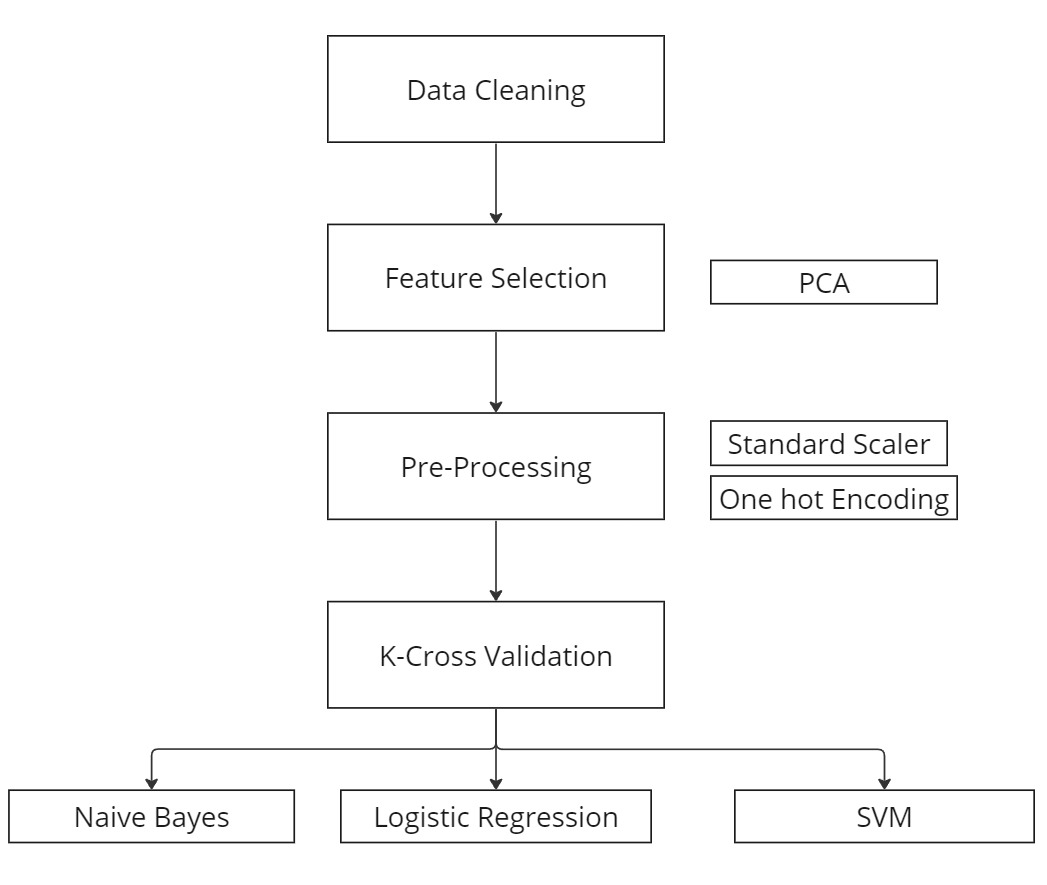
\includegraphics[width=\linewidth]{methodology.jpeg}
\subsection{Gaussian Naive Bayes - Baseline Model}
In the context of using the Naive Bayes technique, an underlying assumption is that all features are independent of each other. However, when we analyzed the distributions of individual features through plotting, we observed that some of these features followed a roughly normal or Gaussian distribution. In contrast, the majority of features exhibited significant skewness, where their distributions were notably skewed to either the left or the right.\\
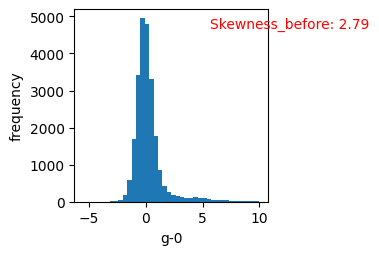
\includegraphics[width=\linewidth]{g_o_before_skewness.png}
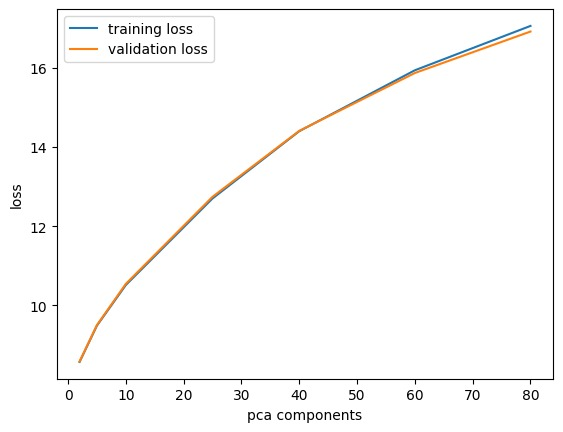
\includegraphics[width=\linewidth]{naive_bayes_pca_component.jpeg}

The Naive Bayes model was employed as the primary analytical tool. In order to enhance its performance and optimize the feature space, Principal Component Analysis (PCA) was utilized as a preprocessing technique. The parameters for PCA were carefully selected through a rigorous cross-validation process to ensure optimal dimensionality reduction.\\
During the experimentation phase, the efficacy of Local Outlier Factor (LOF) as a preprocessing step was evaluated by monitoring the loss curves associated with different LOF parameters. Subsequently, a decision was made to eliminate LOF preprocessing from the model pipeline due to its limited contribution to model performance.

\subsection{Logistic Regression}
In the context of multi-label classification, a conventional approach involves constructing individual classifiers for each label, thereby independently modeling the presence or absence of each label for a given instance. Nonetheless, prior to employing these classifiers, critical preprocessing steps are implemented to improve model performance and robustness.\\
One of the key preprocessing steps is dimensionality reduction using Principal Component Analysis (PCA). PCA is utilized to reduce the dimensionality of the feature space while retaining essential information. The optimal number of principal components, a vital parameter in PCA, is determined through rigorous k-fold cross-validation, with k set to 3. This systematic approach ensures the selection of the most suitable number of principal components, striking a balance between preserving information and reducing dimensionality.\\
Furthermore, for the purpose of enhancing the model's resilience and its ability to identify outliers or anomalies within the dataset, the Local Outlier Factor (LOF) method is initially applied. LOF serves as a valuable tool for detecting data points that deviate significantly from the overall distribution, contributing to the model's overall robustness. However, upon a comprehensive evaluation, it was observed that the model's performance with LOF and without LOF yielded remarkably similar results. As a result, a decision was made to remove the LOF outlier detection method from the model.\\
The optimal parameters for both PCA and LOF were meticulously determined through k-fold cross-validation, ensuring that the selected configurations delivered the best possible outcomes for the particular multi-label classification problem under investigation. This comprehensive approach to preprocessing, coupled with the decision to exclude the LOF method due to its negligible impact on performance, enhances the reliability and efficacy of the ensuing multi-label classification models.\\
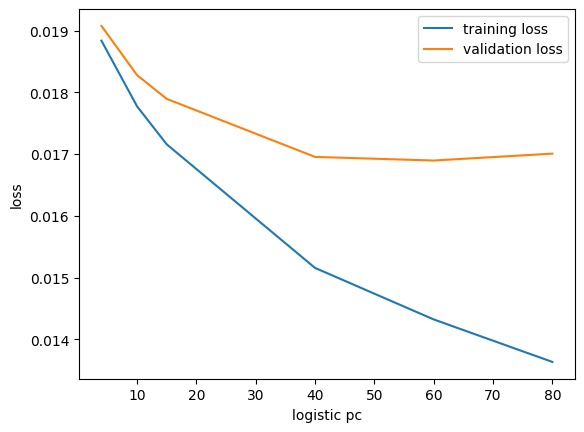
\includegraphics[width=\linewidth]{logistic_pca_comp.jpeg}
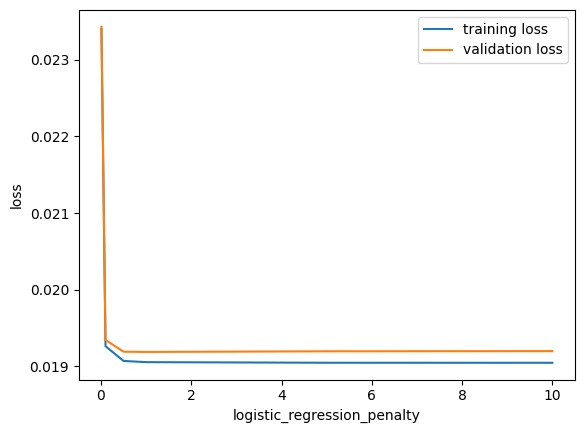
\includegraphics[width=\linewidth]{logistic_penalty.jpeg}
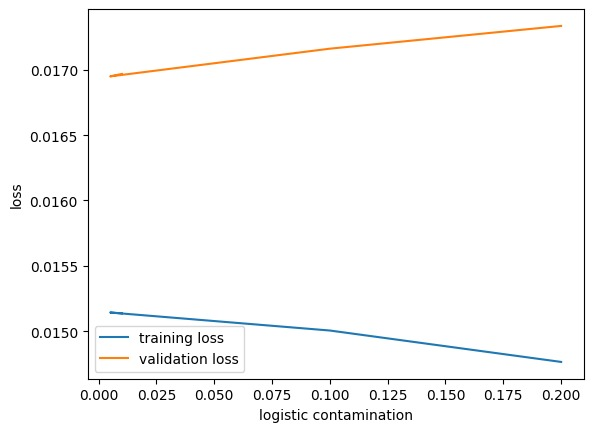
\includegraphics[width=\linewidth]{logistic_lof_contamination.jpeg}

\subsection{SVM}
In our study, an analysis of the dataset revealed inherent non-linearity in class distributions within the feature space. This observation led to the adoption of a Support Vector Machine (SVM) equipped with a Radial Basis Function (RBF) kernel. This kernel choice, known for its prowess in handling non-linear data, leverages its ability to implicitly map the data into a higher-dimensional space where it becomes linearly separable. Recognizing SVM's sensitivity to feature scales, especially with RBF kernels, all features were normalized using StandardScaler to ensure zero mean and unit variance; care was taken to retain genuine data variability and prevent overfitting. The dataset's inherent biases posed another challenge. This was managed by meticulous tuning of SVM hyperparameters, specifically the contamination and neighbors parameters, ensuring the classifier did not unduly favor the majority class. Principal Component Analysis (PCA) was incorporated, given the high dimensionality of post-one-hot encoding. This reduced computational demands and addressed the curse of dimensionality, with varied principal components being tested for optimal balance between efficiency and information retention. Through these strategic preprocessing and tuning steps, the SVM with RBF kernel was adeptly tailored to our specific dataset, aiming for optimal classification performance.
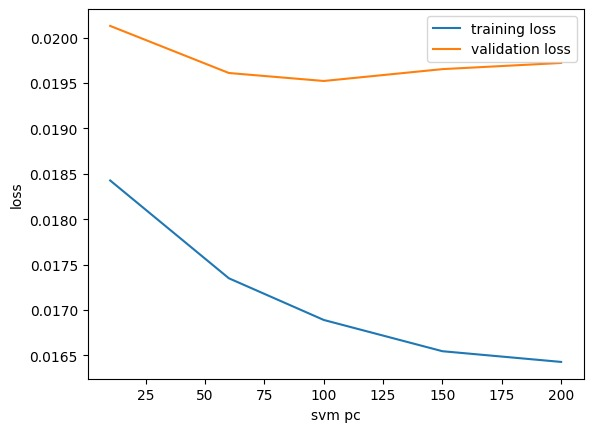
\includegraphics[width=\linewidth]{svm_pc.jpeg}
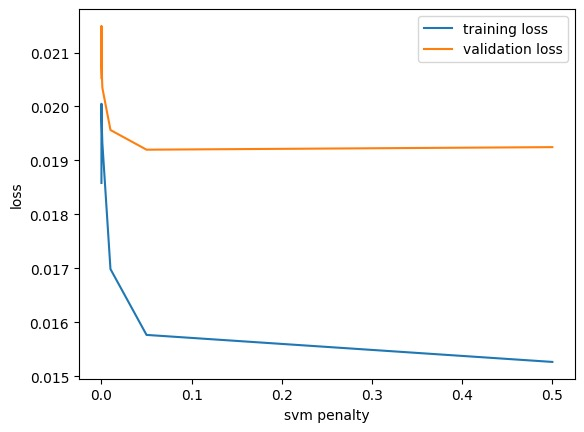
\includegraphics[width=\linewidth]{svm_penalty.jpeg}

\section{Result and Analysis}
Testing Loss from Naive Bayes: 0.17579212096270908
Testing Loss from Logistic Regression: 0.0171752630383298
Testing Loss from Naive SVM: 0.02716435757893583
The Naive Bayes model, as the name suggests, is the most basic of all, and therefore, the performance shown was a log loss of 0.17579212096270908. The number of principal components was 10.  Even though we didn’t have high hopes for it, its simplicity and the quick training time are suitable for a baseline measurement.
Logistic regression showed a log loss of 0.0171752630383298 using Principal components value = 40. As mentioned in the methodology section, it was found using k-fold cross-validation.
The final model we tried was SVM, which showed a log loss of  0.02716435757893583 using the value of the principal component as 30 . 

In light of the research findings, it is observed that the performance loss differential between logistic regression and Support Vector Machines (SVM) is minimal. Consequently, the preference leans toward logistic regression due to its inherent advantages, notably computational efficiency and enhanced interpretability when compared to SVM. This choice is primarily motivated by the computational expediency logistic regression offers, making it a more practical and resource-efficient option for modeling. Furthermore, logistic regression's heightened interpretability, stemming from its linear nature and direct modeling of probabilities, fosters a more transparent and understandable understanding of the relationships between input features and predictive outcomes, facilitating decision-making and domain knowledge integration.

\section{Conclusion}
In conclusion, this research paper was undertaken with the primary objective of developing predictive models for the prediction of Mechanism of Action (MOA). Throughout this study, several algorithms have been proposed and investigated as potential tools for MOA prediction. One notable aspect of this paper is the emphasis placed on explaining the rationale behind selecting specific parameters for the proposed models.\\
This explanatory approach is substantiated by graphical representations, which provide visual insights into the underlying data patterns and the significance of certain model parameters. Such elucidation enhances the transparency and comprehensibility of the model development process, fostering a deeper understanding of the chosen methodologies. In summary, this research endeavor has not only contributed novel algorithms for MOA prediction but has also strived to provide a clear and rational basis for the parameter selections made, thus enriching the interpretability and applicability of the proposed models in the domain of Mechanism of Action prediction. 

\section{References}
[1] H. L. Gururaj, Francesco Flammini, H.A. Chaya Kumari,
G.R. Puneeth, B.R. Sunil Kumar. Classifcation of drugs
based on mechanism of action using machine learning.

[2] Lombardi Alessandro, Polvani Niccolo, Zacchei Filippo.
Department of Mathematics, EPFL, Lausanne, CH.
Mechanism of Action (MoA) Prediction - Kaggle
Competition.

[3] Andreas Mayr, Gunter Klambauer, Thomas Unterthiner,
Marvin Steijaert,b Jorg K. Wegner, Hugo Ceulemans,
Djork-Arne Clevert and Sepp Hochreiter.
Large-scale comparison of machine learning methods for
drug target prediction on ChEMBL




\end{multicols}
\end{document}
